\documentclass[11pt,a4paper]{article}

\usepackage[T1]{fontenc}
\usepackage[utf8]{inputenc}
\IfFileExists{lmodern.sty}{\usepackage{lmodern}}{}
\usepackage[margin=2.5cm]{geometry}
\usepackage{amsmath,amssymb,amsthm,bm}
\usepackage{mathtools}
\usepackage{graphicx}
\usepackage{booktabs}
\usepackage{array}
\usepackage[authoryear,round]{natbib}
\usepackage{xcolor}
\usepackage[colorlinks=true,linkcolor=blue!50!black,citecolor=blue!50!black,urlcolor=blue!50!black]{hyperref}
\usepackage{caption}
\usepackage{enumitem}

\newtheorem{proposition}{Proposition}
\newtheorem{lemma}{Lemma}
\theoremstyle{remark}
\newtheorem{remark}{Remark}

\newcommand{\vect}[1]{\bm{#1}}
\newcommand{\uv}[1]{\hat{\bm{#1}}}
\newcommand{\R}{\mathbb{R}}
\newcommand{\Sph}{\mathbb{S}^2}
\newcommand{\dd}{\,\mathrm{d}}
\newcommand{\T}{^{\mathsf T}}
\newcommand{\Req}{R_{\mathrm{eq}}}
\DeclareMathOperator{\diag}{diag}
\DeclareMathOperator{\tr}{tr}
\DeclareMathOperator{\softplus}{softplus}
\DeclareMathOperator*{\argmax}{arg\,max}

\title{A hybrid Bayesian lightcurve inversion: global nested sampling of spin modes and
Hamiltonian Monte Carlo of a Gaussian-random-field radius model with a principal-axis prior}
\author{Methods note accompanying the \texttt{lcinv.hybrid} prototype}
\date{29 October 2026}

\begin{document}
\maketitle

\begin{abstract}
We present a two-layer Bayesian method for reconstructing the spin state and shape of an asteroid,
with uncertainties, from disk-integrated photometry. The \emph{global layer} explores the full
spin-state space by nested sampling, marginalising a convex Gaussian-image shape with a Laplace
approximation \citep{lcinv_convex2026}. It identifies the posterior modes, typically the mirror pole
pair and any period aliases, together with their approximate mass. The \emph{local layer} replaces
the convex model in each mode by a star-shaped body. Its log-radius field is a truncated, isotropic
Gaussian random field on the sphere with a Mat\'ern-like angular power spectrum and learned
hyperparameters, parametrised in non-centred form. Spherical harmonics on a Gauss--Legendre grid are
exactly orthonormal under the grid quadrature, which keeps the degree structure and the rotation
equivariance about the spin axis intact. Because volume and inertia are explicit radial integrals of
the field, a prior enforcing rotation about the axis of maximum inertia can be imposed directly; this
was not possible in the convex representation. The joint posterior of spin and shape in each mode is
sampled with the No-U-Turn sampler. It uses a singularity-free gnomonic pole chart, an analytically
marginalised photometric nuisance model, and a smoothed limb and terminator. The modes are combined
with weights from a Laplace evidence of the local model. Convexity, ray-traced self-shadowing errors,
MCMC convergence, leave-one-out predictive accuracy and prior sensitivity are reported as diagnostics.
We apply the method to 334 Rubin Observatory measurements of 2003~QN$_{21}$. The inertia prior brings
the spin axis to within $\approx6^\circ$ (median) of the maximum-inertia axis, compared with
$52^\circ$--$88^\circ$ for convex shapes. The fitted noise drops from 17 to 12\,mmag. The diagnostics of a first run traced poor pole mixing to
a twist of the Euler body frame about the spin axis, growing as $\tan\beta$ near the ecliptic poles,
which the shape absorbs. A quaternion body frame defined by parallel transport bounds this twist by
$\tan(d/2)$ around each mode. It removes all divergences, lets the chains cross the ecliptic pole, and
reveals that the pole posterior is an arc perpendicular to the line of sight, 2--10 times wider than the
Euler run suggested. The local evidence favours the prograde solution near $(69^\circ,+59^\circ)$ with
weight 0.99. Non-convex posterior shapes leave a self-shadowing error of $\approx5$\,mmag rms, for
which remedies are given.
\end{abstract}

\tableofcontents

%==========================================================================================
\section{Motivation}
\label{sec:motivation}

The convex inversion of \citet{kaasalainen2001a,kaasalainen2001b}, embedded in a Bayesian framework
with nested sampling \citep{lcinv_convex2026}, handles the multimodality of the spin-state posterior
well. For single-apparition data this multimodality comes from the mirror ambiguity
$(\lambda,\beta)\leftrightarrow(\lambda+180^\circ,-\beta)$ \citep{kaasalainen2006}, period aliases and
nearly degenerate longitudes near the ecliptic poles. Applied to 2003~QN$_{21}$, however, that analysis
exposed two structural limitations.
\begin{enumerate}[nosep]
\item \emph{Physical admissibility.} In the Gaussian-image representation the inertia tensor is not an
  explicit function of the shape parameters. The posterior shapes rotated $52^\circ$--$88^\circ$ away
  from their axis of maximum inertia, so they are not relaxed principal-axis rotators
  \citep{burns1973}.
\item \emph{Shape uncertainty.} The Laplace approximation of the shape posterior at fixed spin is local
  and Gaussian. It cannot represent skewed or multimodal shape uncertainty.
\end{enumerate}
Joint Hamiltonian Monte Carlo over spin and shape addresses the second point, and a radius
representation addresses the first. On its own, however, HMC cannot move between well-separated modes
and provides no evidence for weighting them \citep{betancourt2017}. The hybrid design assigns each task
to the method suited to it. The global layer finds the modes and their approximate mass; the local
layer samples each mode with a physically constrained, more flexible shape model; and a local evidence
recombines the modes (Fig.~\ref{fig:flow}).

\begin{figure}[t]
\centering
\fbox{\begin{minipage}{0.92\linewidth}\small
\textbf{Global layer} (convex Gaussian image, Laplace-marginalised shape, nested sampling over
$(\lambda,\beta,P,\sigma_{\mathrm{jit}})$) $\;\Rightarrow\;$ posterior samples of the pole
$\;\Rightarrow\;$ \textbf{mode identification} on $\Sph$ (\S\ref{sec:modes}) $\;\Rightarrow\;$ for each
mode $k$: \textbf{local model} (\S\ref{sec:local}) $\to$ multi-start MAP $\to$ Laplace evidence
$Z_k$ and covariance $\to$ \textbf{NUTS} with dense mass matrix (\S\ref{sec:nuts}) $\to$
\textbf{diagnostics} (\S\ref{sec:diagnostics}) $\;\Rightarrow\;$ \textbf{mixture}
$\sum_kw_k\,p_k(\cdot\mid\vect y)$ with $w_k\propto Z_k$ (\S\ref{sec:mixture}).
\end{minipage}}
\caption{Structure of the hybrid inversion.}
\label{fig:flow}
\end{figure}

%==========================================================================================
\section{Data, geometry and the global layer}
\label{sec:global}

The photometric reduction, light-time-corrected ephemerides and global layer follow
\citet{lcinv_convex2026}; we restate only the elements needed here.

\paragraph{Data and geometry.} Observations $i=1,\dots,N$ give reduced magnitudes
$y_i=m_i-5\log_{10}(r_i\Delta_i)$, quoted errors $e_i$, bands $b(i)$ and phase angles $\alpha_i$.
The unit vectors $\uv s_i$ (asteroid to Sun) and $\uv e_i$ (asteroid to observer) are in the ecliptic
J2000 frame at the emission time $t_i$. They are computed from JPL Horizons vectors
\citep{giorgini1996}, obtained with \texttt{astro\-query} \citep{ginsburg2019}, with iterated light time.

\paragraph{Global layer.} The convex shape is represented by facet areas
$A_j=w\exp(\sum_{lm}c_{lm}Y_{lm}(\uv n_j))$ on a fixed Gaussian sphere \citep{kaasalainen2001a}. It is
marginalised at each spin state by a Laplace approximation \citep{tierney1986}. The resulting
four-dimensional posterior over $(\lambda,\beta,P,\ln\sigma_{\mathrm{jit}})$ is sampled by nested
sampling \citep{skilling2006,speagle2020}. The rotational phase is gauge-fixed, because for a free shape
it is equivalent to a rotation of the body about the spin axis \citep{lcinv_convex2026}. We use the
equal-weight posterior samples $\{(\lambda_s,\beta_s)\}$ of this layer, and its period-search value
$P_0$ with conservative half-width $\sigma_P$ as the period prior of the local layer.

%==========================================================================================
\section{Mode identification}
\label{sec:modes}

Let $\uv p_s$ be the unit pole vectors of the global samples. Modes are found by greedy density
clustering on the sphere:
\begin{enumerate}[nosep]
\item Among the unassigned samples, choose the seed with the most neighbours within the angular radius
  $r_{\mathrm{core}}=20^\circ$.
\item Define the mode centre as the normalised mean of those neighbours.
\item Assign to the mode all unassigned samples within $r_{\mathrm{mem}}=45^\circ$ of the centre, and
  recompute the centre from the members.
\item Repeat until fewer than 5\% of the samples remain or a maximum number of modes is reached.
\end{enumerate}
The fraction of global samples in each mode is its \emph{global weight}. Explicit mode centres may also
be supplied, for instance from a pole grid search or from other data.

%==========================================================================================
\section{Local model}
\label{sec:local}

\subsection{Star-shaped body and log-radius field}
The body is star-shaped with respect to an interior point:
\begin{equation}
  \mathcal B=\{\rho\,\uv u:\ \uv u\in\Sph,\ 0\le\rho\le r(\uv u)\},\qquad
  r(\uv u)=\exp f(\uv u),\qquad
  f(\uv u)=\sum_{l=l_{\min}}^{l_{\max}}\sum_{m=-l}^{l}a_{lm}\,Y_{lm}(\uv u),
  \label{eq:field}
\end{equation}
where $Y_{lm}$ are real orthonormal spherical harmonics. The degree $l=0$ is omitted because it only
scales the body, which is degenerate with the photometric offsets. The degree $l=1$ is omitted because,
to first order, it translates the body, which does not affect disk-integrated brightness. Hence
$l_{\min}=2$, and we use $l_{\max}=5$, giving $k=(l_{\max}+1)^2-l_{\min}^2=32$ coefficients. A positive
radius is guaranteed by the exponential. This is the parametrisation of the Gaussian random sphere of
\citet{muinonen1998}, here used for the shape of a single body rather than for shape statistics.

\subsection{Gaussian-random-field prior}
\label{sec:grf}
With independent coefficients $a_{lm}\sim\mathcal N(0,\tau_l^2)$, the field $f$ is an isotropic Gaussian
random field on $\Sph$ \citep{marinucci2011}. By the addition theorem its covariance depends only on
the angular separation:
\begin{equation}
  \mathrm{Cov}\bigl[f(\uv u),f(\uv u')\bigr]=\sum_{l=l_{\min}}^{l_{\max}}\frac{2l+1}{4\pi}\,\tau_l^2\,P_l(\uv u\cdot\uv u'),
  \qquad
  \mathrm{Var}\,f=\sum_{l}\frac{2l+1}{4\pi}\tau_l^2 .
  \label{eq:cov}
\end{equation}
We adopt a Mat\'ern-like angular power spectrum. The Whittle--Mat\'ern fields on the sphere have
spectra $\propto(\kappa^2+l(l+1))^{-\nu}$ \citep{lang2015}, which motivates
\begin{equation}
  \tau_l^2(\sigma_f,\ell)=\sigma_f^2\,\frac{4\pi\,s_l}{\sum_{l'}(2l'+1)\,s_{l'}},\qquad
  s_l=\Bigl(1+\frac{l(l+1)}{\ell^2}\Bigr)^{-\nu}.
  \label{eq:spectrum}
\end{equation}
This normalisation makes $\sigma_f$ the pointwise standard deviation of $\ln r$. The \emph{angular scale}
$\ell$ (in degree units) sets the transition to the power-law tail, and the exponent $\nu$ sets the
degree damping and hence the smoothness. We use $\nu=2$ by default and examine $\nu\in\{1.5,3\}$ in a
sensitivity analysis (\S\ref{sec:sensitivity}). The hyperparameters receive weakly informative
log-normal priors,
\begin{equation}
  \ln\sigma_f\sim\mathcal N\bigl(\ln0.15,\,0.5^2\bigr),\qquad \ln\ell\sim\mathcal N\bigl(\ln3,\,0.5^2\bigr).
\end{equation}
The construction resembles a Gaussian-process prior \citep{rasmussen2006} truncated to the band-limited
subspace $l_{\min}\le l\le l_{\max}$.

\paragraph{Non-centred parametrisation.} Because $\tau_l$ depends on the hyperparameters, the centred
form $(a_{lm},\sigma_f,\ell)$ produces the funnel geometry that is notoriously difficult for
Hamiltonian Monte Carlo
\citep{papaspiliopoulos2007,betancourt2015}. We therefore sample standardised coefficients:
\begin{equation}
  a_{lm}=\tau_l(\sigma_f,\ell)\,z_{lm},\qquad z_{lm}\sim\mathcal N(0,1)\ \text{independently}.
  \label{eq:noncentred}
\end{equation}

\subsection{Quadrature grid with exactly orthonormal harmonics}
\label{sec:quadrature}
Integrals over $\Sph$ (mass properties, \S\ref{sec:mass}) and the surface mesh (\S\ref{sec:brightness})
use a product grid. It has $N_\vartheta$ Gauss--Legendre nodes $x_a=\cos\vartheta_a$ with weights
$\omega_a$, and $N_\varphi$ equispaced longitudes $\varphi_b=2\pi b/N_\varphi$, giving the quadrature
\begin{equation}
  \int_{\Sph}g\dd\Omega\approx\sum_{a=1}^{N_\vartheta}\sum_{b=0}^{N_\varphi-1}\omega_a\,\frac{2\pi}{N_\varphi}\,g(\vartheta_a,\varphi_b)
  \equiv\sum_q W_q\,g(\uv u_q).
  \label{eq:quad}
\end{equation}

\begin{proposition}[Discrete orthonormality]
\label{prop:ortho}
If $N_\vartheta\ge l_{\max}+1$ and $N_\varphi\ge2l_{\max}+1$, then for all $l,l'\le l_{\max}$
\begin{equation*}
  \sum_qW_q\,Y_{lm}(\uv u_q)\,Y_{l'm'}(\uv u_q)=\delta_{ll'}\delta_{mm'} .
\end{equation*}
\end{proposition}
\begin{proof}
Write $Y_{lm}=N_{lm}\,P_l^{|m|}(x)\,\Phi_m(\varphi)$, with $\Phi_m\in\{\cos m\varphi,\sin|m|\varphi\}$.
The product $\Phi_m\Phi_{m'}$ is a trigonometric polynomial of degree $\le|m|+|m'|\le2l_{\max}$. The
trapezoidal rule with $N_\varphi$ equispaced nodes integrates trigonometric polynomials of degree
$<N_\varphi$ exactly, so the longitude sum equals the exact integral. That integral vanishes unless
$m=m'$, giving $\pi$ or $2\pi$ otherwise. For $m=m'$, the product $P_l^{|m|}P_{l'}^{|m|}$ is a
polynomial in $x$ of degree $l+l'\le2l_{\max}$; for odd $|m|$ the factors
$(1-x^2)^{1/2}$ pair up into a polynomial. Gauss--Legendre quadrature with $N_\vartheta$ nodes is exact
for polynomials of degree $\le2N_\vartheta-1$, so the latitude sum is exact as well. The discrete inner
product therefore equals the continuous one, which is orthonormal.
\end{proof}
This is the sampling theorem underlying exact spherical transforms \citep[cf.][]{driscoll1994}.
Orthonormality then needs no Gram--Schmidt step across degrees. Such a step would mix degrees, destroy
the per-degree damping of Eq.~\eqref{eq:spectrum}, and break the equivariance of the basis under
rotations about $z$ that underlies the phase gauge. We use $N_\vartheta=16$ and $N_\varphi=32$,
well above the exactness limits ($6$ and $11$); the numerical orthonormality error is
$4\times10^{-15}$.

\subsection{Surface mesh and disk-integrated brightness}
\label{sec:brightness}
The surface is triangulated by connecting neighbouring grid nodes in latitude rings, with two pole
vertices closing the caps. This gives $N_\vartheta N_\varphi+2=514$ vertices $\vect v=r(\uv u)\uv u$ and
$2N_\varphi(N_\vartheta-1)+2N_\varphi=1024$ outward-oriented triangles $t$, with areas $A_t$ and unit
normals $\uv n_t$.

The rotation from ecliptic to body coordinates is
\begin{equation}
  \vect v^{\mathrm b}(t)=\mathsf R_z\bigl(\phi(t)\bigr)\,\mathsf R_y\bigl(\tfrac\pi2-\beta\bigr)\,\mathsf R_z(\lambda)\,\vect v,\qquad
  \phi(t)=\frac{2\pi}{P}\,(t-t_{\mathrm{ref}}),
\end{equation}
with passive rotation matrices and the rotational phase gauge-fixed to zero at the reference epoch
$t_{\mathrm{ref}}$ \citep{lcinv_convex2026}. The disk-integrated brightness under the combined
Lommel--Seeliger and Lambert law \citep{kaasalainen2001b} is
\begin{equation}
  L_i=\sum_tA_t\,S\bigl(\tilde\mu_{it},\tilde\mu_{0,it}\bigr),\qquad
  S(\mu,\mu_0)=\mu\mu_0\Bigl(\frac{1}{\mu+\mu_0}+c_L\Bigr),\quad c_L=0.1,
  \label{eq:brightness}
\end{equation}
where the cosines are smoothed at the limb and terminator:
\begin{equation}
  \tilde\mu_{it}=T\softplus\!\bigl(\uv n_t\cdot\uv e_i^{\,\mathrm b}/T\bigr),\qquad
  \tilde\mu_{0,it}=T\softplus\!\bigl(\uv n_t\cdot\uv s_i^{\,\mathrm b}/T\bigr),\qquad T=0.005 .
  \label{eq:softplus}
\end{equation}
The hard clip $\max(0,\mu)$ makes the log density only piecewise smooth, with kinks whenever a facet
crosses the limb or terminator. Such kinks are a known source of divergent HMC trajectories
\citep{betancourt2017}. With Eq.~\eqref{eq:softplus}, a facet facing away contributes at most
$O(T\ln2)$ in the corresponding cosine.

\paragraph{Discretisation error.} Relative to a $48\times96$ reference mesh, the rms magnitude error of
the $16\times32$ mesh is $2.4$\,mmag over random prior draws, against a fitted noise level of
$\approx12$\,mmag (\S\ref{sec:application}). A $24\times48$ mesh reduces this to 1.0\,mmag at about
twice the cost.

\paragraph{Convexity.} Equation~\eqref{eq:brightness} is exact only for convex bodies. For a non-convex
star-shaped surface it ignores self-shadowing and mutual occlusion. Highly non-convex shapes can produce
lightcurves that a convex model fits well \citep{durech2003}, so non-convexity is often weakly
constrained by photometry. We therefore keep Eq.~\eqref{eq:brightness}, add a weak penalty against
local dents (\S\ref{sec:physical}), and quantify the approximation error by ray tracing
(\S\ref{sec:shadow}).

\subsection{Mass properties}
\label{sec:mass}
For a uniform-density star-shaped body, integrals over the volume reduce to radial integrals:
\begin{equation}
  \int_{\mathcal B}g(\vect x)\dd^3x=\int_{\Sph}\int_0^{r(\uv u)}g(\rho\uv u)\,\rho^2\dd\rho\dd\Omega .
\end{equation}
With $g=1$, $g=\vect x$ and $g=\vect x\vect x\T$ this gives the volume, centroid and second moment,
\begin{equation}
  V=\frac13\int r^3\dd\Omega,\qquad
  \vect c=\frac{1}{4V}\int r^4\uv u\dd\Omega,\qquad
  \mathsf M=\frac15\int r^5\,\uv u\uv u\T\dd\Omega-V\,\vect c\vect c\T,
  \label{eq:mass}
\end{equation}
where $\mathsf M$ is taken about the centroid. The inertia tensor is
$\mathsf I=\tr(\mathsf M)\,\mathsf 1-\mathsf M$. All integrals are evaluated with the quadrature
Eq.~\eqref{eq:quad} and are differentiable in $\vect z$, $\sigma_f$ and $\ell$. For an analytic triaxial
ellipsoid inserted as $r(\uv u)$, Eq.~\eqref{eq:mass} reproduces $V$ and $\diag\mathsf I$ to machine
precision.

\subsection{Physical priors}
\label{sec:physical}

\paragraph{Principal-axis rotation.} A relaxed rotator spins about its axis of maximum inertia
\citep{burns1973}. With $\uv z$ the spin axis, this requires $I_{xz}=I_{yz}=0$ and
$I_{zz}\ge\lambda_{\max}(\mathsf I_{xy})$, where
\begin{equation}
  \lambda_{\max}(\mathsf I_{xy})=\tfrac12(I_{xx}+I_{yy})+\sqrt{\tfrac14(I_{xx}-I_{yy})^2+I_{xy}^2}
\end{equation}
is the largest eigenvalue of the equatorial block. We impose these conditions softly:
\begin{equation}
  \ln\pi_{\mathrm{inertia}}=-\frac12\left(\frac{I_{xz}/I_{zz}}{s_{\mathrm{off}}}\right)^{\!2}
  -\frac12\left(\frac{I_{yz}/I_{zz}}{s_{\mathrm{off}}}\right)^{\!2}
  -\frac12\left[\softplus\!\left(\frac{d}{s_{\mathrm{ord}}}\right)\right]^2,\qquad
  d=\frac{\lambda_{\max}(\mathsf I_{xy})-I_{zz}}{I_{zz}},
  \label{eq:inertiaprior}
\end{equation}
with $s_{\mathrm{off}}=s_{\mathrm{ord}}=0.005$. By first-order perturbation theory the
maximum-inertia axis is tilted from $\uv z$ by
\begin{equation}
  \delta\approx\left(\frac{I_{xz}}{I_{zz}-I_{xx}},\,\frac{I_{yz}}{I_{zz}-I_{yy}}\right),
\end{equation}
so the prior in Eq.~\eqref{eq:inertiaprior} constrains the tilt to
$\sim s_{\mathrm{off}}\,I_{zz}/(I_{zz}-I_2)$, where $I_2$ is the second-largest moment. When the two
largest moments are nearly equal, the maximum-inertia axis is ill-defined. The tilt angle is then a
poor diagnostic, which is why we always report it together with the moment gap.

\paragraph{Convexity penalty.} For each grid vertex $\vect v_q$ with ring neighbours
$\{\vect v_{q'}\}$ (east, west, south, north), the local outward bulge is
$b_q=(\vect v_q-\overline{\vect v}_{\mathcal N(q)})\cdot\uv u_q/\bar r$. It is negative at a dent. We
add the weak penalty
\begin{equation}
  \ln\pi_{\mathrm{cvx}}=-\frac{1}{2s_{\mathrm{cvx}}^2}\sum_q\bigl[\max(0,-b_q)\bigr]^2,\qquad s_{\mathrm{cvx}}=0.02 .
\end{equation}
These physical terms are constraint factors rather than normalised priors. Their normalising constants
are identical across modes, so they cancel in the mode weights of \S\ref{sec:mixture}.

\subsection{Spin parameters}
\label{sec:spin}

\paragraph{Gnomonic pole chart.} Within mode $k$, with centre $\uv p_k$ and an orthonormal tangent basis
$(\uv e_1,\uv e_2)$, the pole is
\begin{equation}
  \uv p(d_1,d_2)=\frac{\uv p_k+d_1\uv e_1+d_2\uv e_2}{\lVert\uv p_k+d_1\uv e_1+d_2\uv e_2\rVert},
  \qquad(d_1,d_2)\in\R^2 .
\end{equation}
This chart covers the open hemisphere centred on $\uv p_k$, has no singularity at $|\beta|=90^\circ$ (the
cause of poor nested-sampling efficiency in the polar caps; \citealp{lcinv_convex2026}), and cannot
reach the mirror mode. A uniform prior on the sphere transforms with the Jacobian of the gnomonic
projection \citep{snyder1987}.

\begin{lemma}
In the gnomonic chart, $\dd\Omega=(1+\rho^2)^{-3/2}\dd d_1\dd d_2$ with $\rho^2=d_1^2+d_2^2$. Hence a
uniform prior on the sphere has log density $-\ln4\pi-\tfrac32\ln(1+\rho^2)$ in $(d_1,d_2)$.
\end{lemma}
\begin{proof}
A tangent-plane point at radius $\rho$ and azimuth $\psi$ maps to the unit vector at central angle
$\theta=\arctan\rho$ and the same azimuth. Then $\dd\Omega=\sin\theta\dd\theta\dd\psi$, with
$\sin\theta=\rho/\sqrt{1+\rho^2}$ and $\dd\theta=\dd\rho/(1+\rho^2)$, so
$\dd\Omega=\rho(1+\rho^2)^{-3/2}\dd\rho\dd\psi=(1+\rho^2)^{-3/2}\dd d_1\dd d_2$.
\end{proof}

\paragraph{Body frame: quaternion parallel transport.} The orientation of the body at $t_{\mathrm{ref}}$
is a rotation $\mathsf R_0\in SO(3)$ taking ecliptic vectors to body coordinates, with
$\mathsf R_0\uv p=\uv z$. Only two of its three degrees of freedom are identifiable. The pole
$\uv p\in\Sph$ is one point of the quotient $SO(3)/SO(2)$; the remaining twist about the spin axis is the
rotational-phase gauge, which the shape harmonics absorb exactly. A frame construction is therefore a
choice of \emph{section}: a smooth map $\uv p\mapsto\mathsf R_0(\uv p)$. The classical Euler section
$\mathsf R_0=\mathsf R_y(\tfrac\pi2-\beta)\mathsf R_z(\lambda)$ behaves badly near the ecliptic poles.

\begin{proposition}[Twist of the Euler section]
\label{prop:twist}
Under $\lambda\mapsto\lambda+\dd\lambda$ at fixed $\beta$, the Euler frame rotates by the angular
displacement $\uv z_{\mathrm{ecl}}\dd\lambda$. Its component about the spin axis (the twist) is
$\sin\beta\dd\lambda$, while the pole moves by $\cos\beta\dd\lambda$. The twist per unit pole
displacement is therefore $\tan\beta$, which diverges at the ecliptic poles.
\end{proposition}
\begin{proof}
$\mathsf R_z(\lambda)$ is a rotation about the ecliptic $\uv z_{\mathrm{ecl}}$, and $\mathsf R_y$ does
not depend on $\lambda$, so the incremental rotation is about $\uv z_{\mathrm{ecl}}$ by $\dd\lambda$. Its
projection onto $\uv p$ is $(\uv z_{\mathrm{ecl}}\cdot\uv p)\dd\lambda=\sin\beta\dd\lambda$, and
$\lVert\partial\uv p/\partial\lambda\rVert=\cos\beta$.
\end{proof}

Since a twist is absorbed by rotating the shape harmonics, Proposition~\ref{prop:twist} implies a
near-flat, curved ridge in $(\lambda,\vect z)$ space for poles near the ecliptic poles. This is the
geometry that causes long NUTS trajectories and poor mixing (\S\ref{sec:application}). We therefore
build $\mathsf R_0$ with unit quaternions by \emph{parallel transport} from the mode centre:
\begin{equation}
  \mathsf R_0(\uv p)=\mathsf R(q_k)\,\mathsf R\bigl(q_t(\uv p)\bigr),\qquad
  q_t(\uv p)=\frac{\bigl(1+\uv p\cdot\uv p_k,\ \uv p\times\uv p_k\bigr)}{\bigl\lVert\bigl(1+\uv p\cdot\uv p_k,\ \uv p\times\uv p_k\bigr)\bigr\rVert},
  \label{eq:quatframe}
\end{equation}
where $q=(w,\vect v)$ denotes a quaternion and $\mathsf R(q)$ its rotation matrix. The tilt $q_t$ is
the minimal rotation taking $\uv p$ onto $\uv p_k$; the half-angle formula needs no trigonometric
functions. The fixed quaternion $q_k$ takes $\uv p_k$ onto $\uv z$, so $\mathsf R_0(\uv p)\uv p=\uv z$.

\begin{proposition}[Bounded twist of the parallel-transport section]
\label{prop:qtwist}
Let $d$ be the angular distance of $\uv p$ from the mode centre $\uv p_k$. Under a displacement
$\dd\uv p$, the section of Eq.~\eqref{eq:quatframe} twists about the spin axis by at most
$\tan(d/2)\,\lVert\dd\uv p\rVert$. The twist vanishes for radial displacements and at the centre
itself, and attains the bound for transverse displacements.
\end{proposition}
\begin{proof}
Use geodesic polar coordinates $(d,\psi)$ centred on $\uv p_k$. Transporting the reference frame from
$\uv p_k$ along the geodesic to $\uv p$ defines an orthonormal frame field. For radial displacements
($\dd\psi=0$) the frame is parallel along the geodesic, so there is no twist. For transverse
displacements, the twist relative to parallel transport is given by the connection one-form of this
frame field on the unit sphere, $\omega=(1-\cos d)\dd\psi$; this is the holonomy of the geodesic
triangle with vertices $\uv p_k$, $\uv p$ and $\uv p+\dd\uv p$. The displacement is
$\lVert\dd\uv p\rVert=\sin d\dd\psi$, so the ratio is $(1-\cos d)/\sin d=\tan(d/2)$.
\end{proof}

The Euler section is the analogous construction centred on the \emph{ecliptic} pole. Its connection
one-form is $\sin\beta\dd\lambda$, which gives the ratio $\tan\beta$ of
Proposition~\ref{prop:twist}. The parallel-transport section therefore moves the coordinate centre to
the mode, where the twist rate is small: at most $0.18$ within $20^\circ$ of the centre, independent of
ecliptic latitude. The residual twist is a smooth, bounded rotation rather than a divergence.

The section of Eq.~\eqref{eq:quatframe} is smooth on the whole sphere except at the antipode
$-\uv p_k$, which lies outside the hemisphere covered by the gnomonic chart. A fully free quaternion,
with three rotational degrees of freedom, would instead reintroduce the exactly flat gauge direction, as
well as the sign ambiguity $q\sim-q$ and a norm constraint. Numerically, at the mode centre the twist per unit pole displacement is below $10^{-5}$ for the
quaternion section at all latitudes, against 5.7 at $\beta=80^\circ$ and 60 at $\beta=89^\circ$ for
the Euler section, as predicted by $\tan\beta$. Off-centre, the quaternion section reproduces
$\tan(d/2)$ to four decimals for $d$ up to 0.5\,rad. The previous Euler
results remain available through an option.

\paragraph{Period, phase and jitter.} The period is non-centred, $P=P_0+\sigma_P z_P$ with
$z_P\sim\mathcal N(0,1)$, where $P_0$ and $\sigma_P$ are the period-search value and its conservative
half-width. The rotational phase is gauge-fixed (Proposition~1 of \citealp{lcinv_convex2026}). Within a
mode, all draws therefore share one body frame, and shapes can be averaged without registration. The
jitter has prior $\ln\sigma_{\mathrm{jit}}\sim\mathcal N(\ln0.015,1)$.

\subsection{Likelihood with analytically marginalised nuisance parameters}
\label{sec:likelihood}
The model magnitudes are $\mu_i=-2.5\log_{10}L_i+\mathsf X_i\vect\eta$, where $\vect\eta$ contains one
offset per band and a linear phase-angle slope. With $\sigma_i^2=e_i^2+\sigma_{\mathrm{jit}}^2$,
$\mathsf W=\diag(\sigma_i^{-2})$ and $\vect y^\star=\vect y+2.5\log_{10}\vect L$, integrating
$\vect\eta\in\R^p$ against a flat prior gives
\begin{equation}
  \ln p(\vect y\mid\vect x)=-\frac12\,\vect r\T\mathsf W\vect r-\frac12\sum_i\ln(2\pi\sigma_i^2)
  -\frac12\ln\det\bigl(\mathsf X\T\mathsf W\mathsf X\bigr)+\frac p2\ln2\pi,
  \label{eq:marglik}
\end{equation}
with $\vect r=\vect y^\star-\mathsf X\hat{\vect\eta}$ and
$\hat{\vect\eta}=(\mathsf X\T\mathsf W\mathsf X)^{-1}\mathsf X\T\mathsf W\vect y^\star$. This follows from
completing the square in $\vect\eta$. The determinant term depends on the parameters through
$\sigma_{\mathrm{jit}}$ and corrects the profile likelihood used in \citet{lcinv_convex2026}. The flat
prior is improper, but its constant is common to all modes and cancels in the mode weights. For
leave-one-out cross-validation we store the pointwise terms
$\ln\mathcal N(y_i^\star\mid\mathsf X_i\hat{\vect\eta},\sigma_i^2)$. These are evaluated at the
draw-specific $\hat{\vect\eta}$ and are thus an approximation to the pointwise marginal likelihood.

\subsection{Full local posterior}
The unconstrained parameter vector is
$\vect x=(d_1,d_2,z_P,\ln\sigma_{\mathrm{jit}},\ln\sigma_f,\ln\ell,\vect z)\in\R^{6+k}$, of dimension 38.
Its log density is
\begin{equation}
  \ln p(\vect x\mid\vect y)=\ln p(\vect y\mid\vect x)+\ln\pi(\vect x)+\ln\pi_{\mathrm{inertia}}+\ln\pi_{\mathrm{cvx}}+\text{const},
  \label{eq:logpost}
\end{equation}
where $\ln\pi(\vect x)$ collects the gnomonic pole prior, the standard normal priors on $z_P$ and
$\vect z$, and the priors on $\ln\sigma_{\mathrm{jit}}$, $\ln\sigma_f$ and $\ln\ell$. The whole of
Eq.~\eqref{eq:logpost} is implemented in JAX \citep{jax2018}; gradients and Hessians are exact.

%==========================================================================================
\section{Inference within a mode}
\label{sec:nuts}

\subsection{Maximum a posteriori and Laplace approximation}
The MAP is found by L-BFGS \citep{liu1989,optax2020} from several starting points. They differ in the
initial equatorial elongation, $a_{2,2}=-0.25\cos2\psi_j$ and $a_{2,-2}=-0.25\sin2\psi_j$ with
$\psi_j=j\pi/n_s$, because elongation orientations define separate basins. Convergence requires a small
gradient norm and a positive-definite Hessian $\mathsf H=-\nabla^2\ln p$. A run stopped after a fixed
small number of iterations can sit on a saddle. Clipping its negative curvatures would inflate the
Laplace evidence by tens of nats, so such cases are iterated further (2000 iterations by default) and
flagged if they persist.

The Laplace approximation \citep{tierney1986}
\begin{equation}
  \ln Z_k\approx\ln p(\vect y,\hat{\vect x}_k)+\frac{d}{2}\ln2\pi-\frac12\ln\det\mathsf H_k
  \label{eq:laplaceZ}
\end{equation}
provides the evidence of mode $k$ (\S\ref{sec:mixture}). The covariance $\mathsf H_k^{-1}$ supplies the
NUTS initial points ($\hat{\vect x}_k$ plus $0.3$ times Laplace draws) and the initial dense mass matrix.

\subsection{No-U-Turn sampling}
Hamiltonian Monte Carlo \citep{neal2011,betancourt2017} augments $\vect x$ with momenta $\vect p$ and
simulates
\begin{equation}
  \mathcal H(\vect x,\vect p)=-\ln p(\vect x\mid\vect y)+\tfrac12\,\vect p\T\mathsf M^{-1}\vect p
\end{equation}
with the leapfrog integrator. The No-U-Turn sampler \citep{hoffman2014} builds trajectories by
recursive doubling until a U-turn criterion is met or the maximum tree depth is reached, and samples a
state from the trajectory. The step size is adapted by dual averaging \citep{nesterov2009} to a target
acceptance probability of $0.9$. The dense inverse mass matrix $\mathsf M^{-1}$ is initialised with
$\mathsf H_k^{-1}$ and re-estimated from the warm-up draws. A divergence is recorded whenever the
energy error of a trajectory exceeds a large threshold; divergences signal regions of high curvature
that the sampler cannot resolve. We use NumPyro \citep{phan2019,bingham2019} with a potential function
equal to $-\ln p(\vect x\mid\vect y)$, two chains in parallel, 400 warm-up and 400 sampling iterations,
and a maximum tree depth of 7.

%==========================================================================================
\section{Combination of modes}
\label{sec:mixture}

With well-separated modes, the posterior is approximately the mixture
\begin{equation}
  p(\vect\vartheta\mid\vect y)\approx\sum_kw_k\,p_k(\vect\vartheta\mid\vect y),\qquad
  w_k=\frac{Z_k}{\sum_jZ_j},
  \label{eq:mixture}
\end{equation}
where $p_k$ is the NUTS posterior of mode $k$ and $Z_k$ its evidence (Eq.~\ref{eq:laplaceZ}). Ratios
$Z_k/Z_j$ are Bayes factors between the modes \citep{kass1995}. Because the gnomonic chart restricts each
local model to the hemisphere around $\uv p_k$, $Z_k$ integrates the prior only over that hemisphere.
For posterior mass concentrated near the centre this is exact up to a negligible overlap.

We report the global-layer fractions alongside $w_k$. The two sets of weights refer to different shape
models, convex versus radius field, so a difference between them is itself informative. Predictive
stacking \citep{yao2018} is an alternative when the modes are viewed as competing models rather than
regions of one posterior.

\begin{remark}
The Laplace evidence inherits the local Gaussian approximation. If a mode's posterior is markedly
non-Gaussian, for example skewed in $\sigma_f$, the weights carry corresponding uncertainty. A
thermodynamic or nested-sampling evidence of the local model in each mode would remove this
approximation at higher cost.
\end{remark}

%==========================================================================================
\section{Diagnostics}
\label{sec:diagnostics}

\subsection{Convergence}
For each scalar quantity we compute the rank-normalised split-$\widehat R$ of \citet{vehtari2021}. Each
chain is split in half, the pooled draws are replaced by normal scores $z=\Phi^{-1}\bigl((\mathrm{rank}-3/8)/(S+1/4)\bigr)$,
where $S$ is the total number of draws, and the classical potential scale reduction
\begin{equation}
  \widehat R=\sqrt{\frac{\frac{n-1}{n}W+\frac1nB}{W}}
\end{equation}
is evaluated, with $W$ and $B$ the within- and between-chain variances. The same is done for the
folded draws $|\theta-\mathrm{median}|$, and the larger value is reported. The pole longitude is first
unwrapped about its circular mean. The bulk effective sample size uses the chain-averaged
autocorrelation truncated by Geyer's initial positive sequence \citep{geyer1992}. We report divergences
and mean trajectory lengths, and export ArviZ data \citep{kumar2019} with a \texttt{log\_likelihood}
group. Pareto-smoothed importance-sampling leave-one-out cross-validation
\citep{vehtari2017,vehtari2024} is computed when available.

\subsection{Convexity}
For a draw with mesh vertices $\{\vect v\}$ and facets $(\uv n_t,\vect v_{t,0})$, the maximum protrusion
\begin{equation}
  \Pi=\frac{1}{\Req}\max_t\max_{\vect v}\,\uv n_t\cdot(\vect v-\vect v_{t,0}),\qquad \Req=\Bigl(\frac{3V}{4\pi}\Bigr)^{1/3},
\end{equation}
vanishes exactly for a convex polyhedron. We also report the area fraction of facets with protrusion
above $10^{-3}\Req$.

\subsection{Self-shadowing error by ray tracing}
\label{sec:shadow}
For selected draws and epochs, rays are cast from each contributing facet centre, offset slightly along
its normal, towards the Sun and towards the observer. Intersections with all triangles are tested with
the M\"oller--Trumbore algorithm \citep{moller1997}. For origin $\vect o$, direction $\uv d$ and
triangle $(\vect v_0,\vect v_1,\vect v_2)$, define $\vect e_1=\vect v_1-\vect v_0$,
$\vect e_2=\vect v_2-\vect v_0$, $\vect h=\uv d\times\vect e_2$, $a=\vect e_1\cdot\vect h$,
$\vect s=\vect o-\vect v_0$ and $\vect q=\vect s\times\vect e_1$. A hit occurs when
\begin{equation}
  u=\frac{\vect s\cdot\vect h}{a}\ge0,\quad v=\frac{\uv d\cdot\vect q}{a}\ge0,\quad u+v\le1,\quad
  t=\frac{\vect e_2\cdot\vect q}{a}>\epsilon .
\end{equation}
Facets that are shadowed or occluded are removed from the sum, and the error of the convex
approximation is
\begin{equation}
  \Delta m_i=2.5\log_{10}\frac{L_i^{\mathrm{facet\ sum}}}{L_i^{\mathrm{ray\ traced}}}\ \ge0 .
\end{equation}
This error is compared with the noise level $\sigma_i$: an rms $\Delta m$ well below the jitter
justifies the facet sum.

\subsection{Prior sensitivity}
\label{sec:sensitivity}
For each mode, the MAP and Laplace evidence are recomputed under weaker ($\nu=1.5$) and stronger ($\nu=3$)
degree damping and under a tighter amplitude prior ($\sigma_f$ prior median $0.08$). We report the MAP
poles and the implied mode weights. Stronger shrinkage towards a sphere reduces the attainable
amplitude, and the spin state may compensate by moving towards equator-on aspects. This sensitivity is
part of the result for single-apparition data.

%==========================================================================================
\section{Application to 2003~QN$_{21}$}
\label{sec:application}

We report two runs with identical data, priors and sampler settings. The first used the legacy Euler body
frame (\S\S\ref{sec:app_data}--\ref{sec:app_sens}). Its diagnostics revealed the twist coupling of
Proposition~\ref{prop:twist}, which motivated the quaternion frame of Eq.~\eqref{eq:quatframe}. The second
run uses that frame and is the adopted result (\S\ref{sec:app_quat}).

\subsection{Data and global modes}
\label{sec:app_data}
The data are 334 $gri$ measurements from five nights of Rubin Observatory photometry
(2026 February 23--27), with phase angle $10.2^\circ\to8.9^\circ$. The global layer
\citep{lcinv_convex2026} yields the period prior $P_0=3.24826$\,h, $\sigma_P=0.00142$\,h, and two pole
modes:
\begin{itemize}[nosep]
\item mode~1 (retrograde): centre $(\lambda,\beta)=(244^\circ,-73^\circ)$, global weight 0.53;
\item mode~2 (prograde): centre $(66^\circ,+71^\circ)$, global weight 0.47.
\end{itemize}
These are the mirror pair expected for near-coplanar viewing \citep{kaasalainen2006}.

\subsection{MAP and evidence}
Multi-start L-BFGS reached $\ln p=840.20$ (mode~1, gradient norm $2.9\times10^{-2}$) and $842.18$
(mode~2, $8.7\times10^{-6}$). Both Hessians are positive definite. The four starts differed by up to
17~nats in mode~1 and 11~nats in mode~2, which confirms that the elongation orientation defines
distinct basins. The Laplace evidences are $\ln Z_1=768.55$ and $\ln Z_2=770.09$, giving local mode
weights $w_1=0.18$ and $w_2=0.82$. This reverses the near-equal split of the global layer.

\subsection{Sampling and convergence}
Table~\ref{tab:conv} summarises the NUTS runs (two chains, 400 warm-up and 400 draws each). The period,
jitter and inertia-tilt quantities mix well ($\widehat R\le1.04$, ESS 400--800). The pole does not: in
mode~1 $\widehat R=1.13$ ($\lambda$) and $1.19$ ($\beta$); in mode~2 $\widehat R=1.29$ for $\lambda$,
with ESS of 12. Mode~1 also exhausted the maximum tree depth (mean 127 leapfrog steps), whereas mode~2
used a mean of 71 steps with 6 divergences. The pole intervals below are therefore lower bounds on the
true spread; \S\ref{sec:discussion} identifies the cause.

\begin{table}[t]
\centering
\caption{Convergence diagnostics per mode: rank-normalised split $\widehat R$ / bulk ESS from 800 draws.}
\label{tab:conv}
\small
\begin{tabular}{@{}lcc@{}}
\toprule
Quantity & Mode 1 (retrograde) & Mode 2 (prograde)\\
\midrule
$\lambda$ & 1.128 / 39 & 1.291 / 12\\
$\beta$ & 1.190 / 77 & 1.068 / 22\\
$P$ & 1.003 / 436 & 1.002 / 800\\
$\sigma_{\mathrm{jit}}$ & 1.037 / 410 & 1.006 / 800\\
$\sigma_f$ & 1.063 / 49 & 1.002 / 340\\
$\ell$ & 1.011 / 50 & 1.002 / 387\\
spin--$I_{\max}$ tilt & 1.010 / 589 & 0.999 / 800\\
Divergences; mean leapfrog steps & 1; 127 & 6; 71\\
NUTS wall time (2 parallel chains) & 1967\,s & 1462\,s\\
\bottomrule
\end{tabular}
\end{table}

\begin{figure}[t]
  \centering
  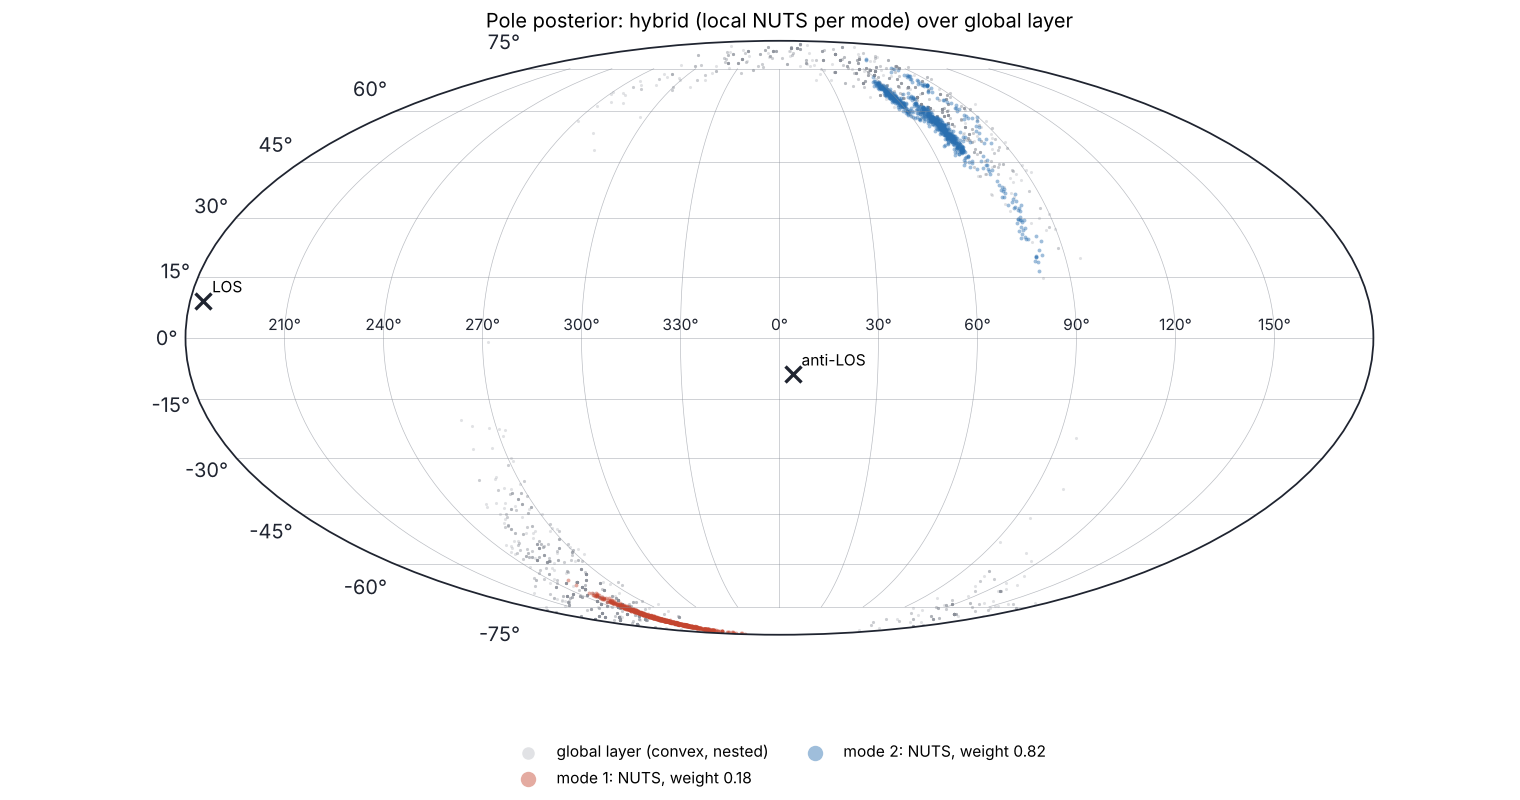
\includegraphics[width=\linewidth]{figures/fig_pole_hybrid.png}
  \caption{Pole posterior of the hybrid model. Coloured points are NUTS draws of the two local modes,
  labelled with their Laplace-evidence weights. Grey points are the global-layer (convex, nested
  sampling) posterior. Crosses mark the line of sight and its antipode.}
  \label{fig:pole}
\end{figure}

\begin{figure}[t]
  \centering
  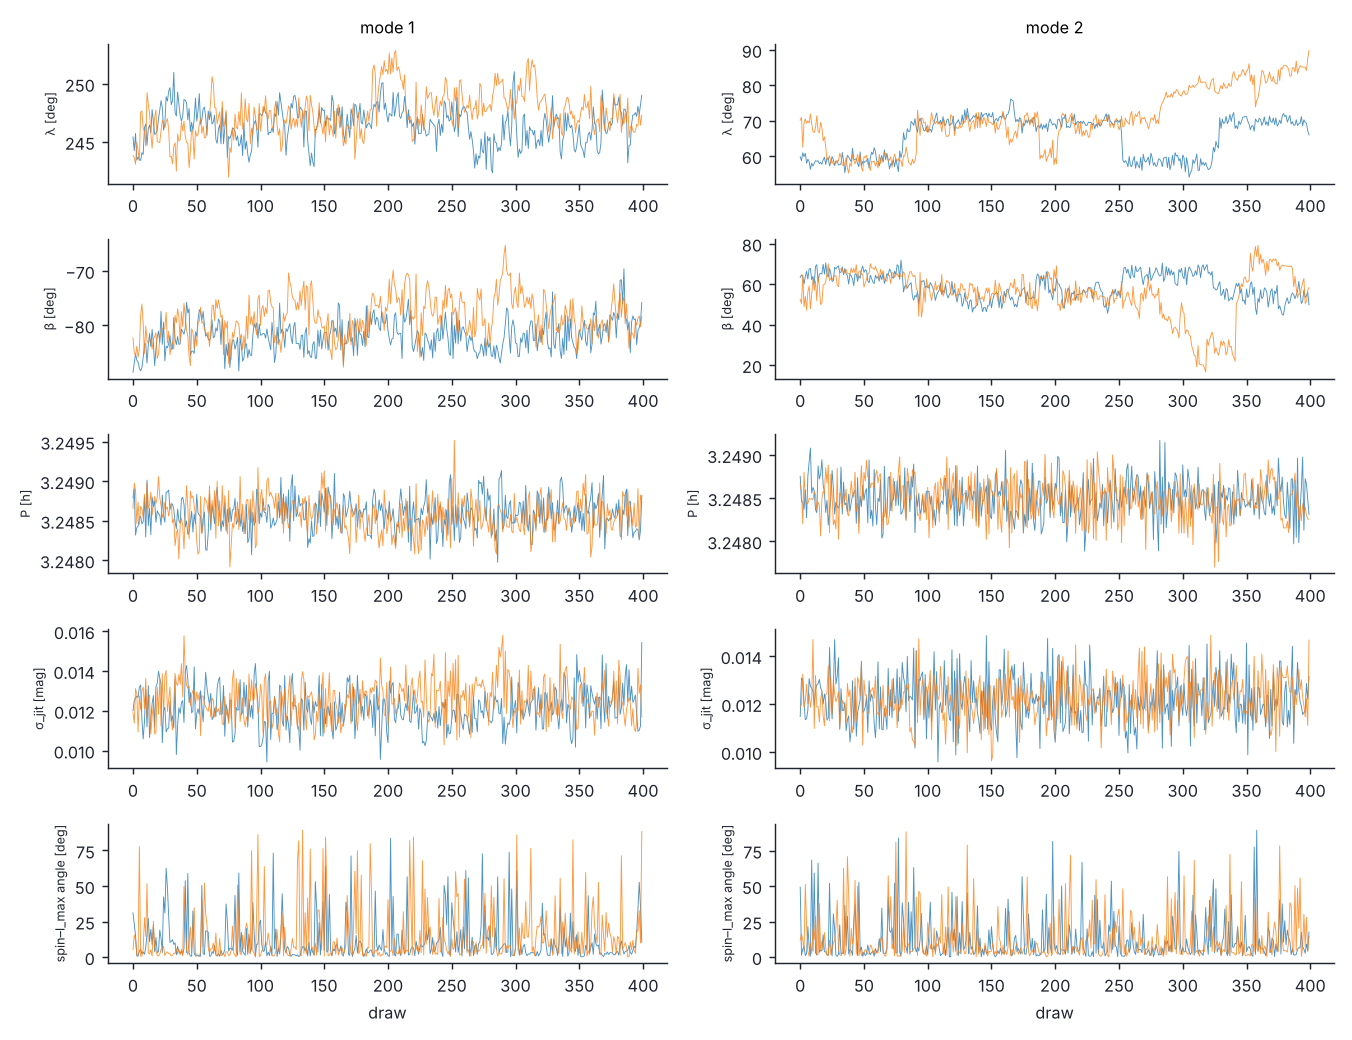
\includegraphics[width=0.62\linewidth]{figures/fig_traces.png}
  \caption{NUTS traces of the pole, period, jitter and spin--maximum-inertia tilt for both modes. The
  slow drift of $\lambda$ and $\beta$ contrasts with the rapid mixing of $P$ and $\sigma_{\mathrm{jit}}$.}
  \label{fig:traces}
\end{figure}

\subsection{Posterior summaries}
Table~\ref{tab:post} lists the posterior summaries and Fig.~\ref{fig:pole} shows the pole draws. The
prograde mode moves from the global centre $(67^\circ,+71^\circ)$ to $(69^\circ,+57^\circ)$ and extends
along the great circle perpendicular to the line of sight to $\beta\approx+20^\circ$. The retrograde
mode tightens near $(247^\circ,-80^\circ)$. Both modes agree on the period, $3.2485\pm0.0002$\,h, which
lies about $1\sigma$ above the global estimate of $3.24828$\,h. They also agree on the jitter,
$12.2$\,mmag, compared with $17.2$\,mmag for the convex model. The posterior-predictive lightcurves
(Fig.~\ref{fig:lc}) follow all five nights. The largest residuals are the faint $i$-band points at the
start of night~1, as in the convex analysis.

\begin{table}[t]
\centering
\caption{Posterior summaries (median and 16th--84th percentiles). Pole radii enclose 68/95\% of the
draws around the mean pole; given the convergence diagnostics they are lower bounds.}
\label{tab:post}
\small
\begin{tabular}{@{}>{\raggedright\arraybackslash}p{0.33\linewidth}>{\raggedright\arraybackslash}p{0.30\linewidth}>{\raggedright\arraybackslash}p{0.30\linewidth}@{}}
\toprule
Quantity & Mode 1 (retrograde) & Mode 2 (prograde)\\
\midrule
Weight: local (global) & 0.18 (0.53) & 0.82 (0.47)\\
Mean pole $(\lambda,\beta)$ & $(247.3^\circ,-80.3^\circ)$ & $(68.9^\circ,+57.2^\circ)$\\
Pole radius 68\% / 95\% & $3.8^\circ$ / $7.5^\circ$ & $9.0^\circ$ / $22.0^\circ$\\
Sidereal period [h] & 3.24858 (3.24837--3.24880) & 3.24849 (3.24826--3.24873)\\
Jitter [mmag] & 12.3 (11.3--13.4) & 12.2 (11.2--13.1)\\
$\sigma_f$ & 0.105 (0.092--0.121) & 0.108 (0.093--0.125)\\
$\ell$ & 1.81 (1.24--2.56) & 1.70 (1.20--2.35)\\
Principal moments (median) & $0.667:0.966:1$ & $0.662:0.965:1$\\
Moment gap $1-I_2/I_3$ & 0.034 (0.011--0.074) & 0.035 (0.012--0.068)\\
Spin--$I_{\max}$ tilt & $5.8^\circ$ ($1.6^\circ$--$23.5^\circ$) & $5.6^\circ$ ($1.8^\circ$--$24.1^\circ$)\\
Median $\sigma_r$ & 4.0\%\,$\Req$ & 4.9\%\,$\Req$\\
PSIS-LOO $\mathrm{elpd}$ ($\max\hat k$) & $872.4\pm14.2$ (0.39) & $874.7\pm14.2$ (0.35)\\
\bottomrule
\end{tabular}
\end{table}

\begin{figure}[t]
  \centering
  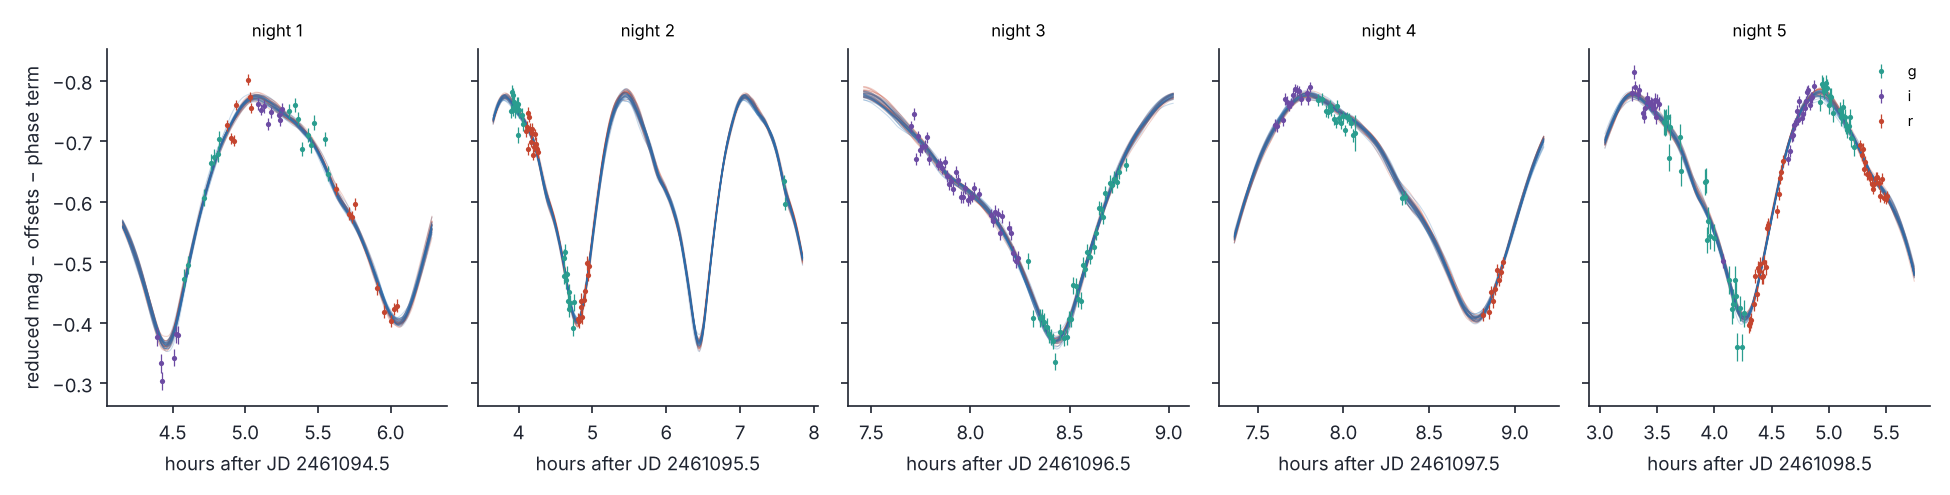
\includegraphics[width=\linewidth]{figures/fig_lightcurves_hybrid.png}
  \caption{Reduced photometry per night with offsets and phase term removed (posterior medians of the
  main mode), and posterior-predictive $r$-band curves from 25 draws of each mode (red: mode~1; blue:
  mode~2).}
  \label{fig:lc}
\end{figure}

\subsection{Shape, inertia and physical checks}
Both modes yield elongated shapes. The normalised principal moments are $\approx0.66:0.97:1$, so the
long axis lies in the equatorial plane and the two largest moments are nearly equal. The inertia prior
is effective: the median tilt between the spin axis and the maximum-inertia axis is $\approx6^\circ$,
compared with $52^\circ$--$88^\circ$ in the convex analysis. Its 84th percentile ($\approx24^\circ$)
reflects the small moment gap of $\approx3.5\%$, which makes the maximum-inertia axis ill-defined
(\S\ref{sec:physical}).

The radius uncertainty (Fig.~\ref{fig:rmaps}) is 3--6\% of $\Req$ (mode~1) and 3--9\% (mode~2). It is
largest at the ends of the long axis in mode~2, where the poorly mixed pole longitude and the shape
orientation trade off.

The facet-plane test finds clearly non-convex shapes. The median maximum protrusion is $0.17\,\Req$
(maximum $0.28\,\Req$), and about two thirds of the surface area lies on facets with protrusion above
$10^{-3}\Req$. Ray tracing of four draws at 30 epochs per mode gives self-shadowing errors of the facet
sum of $6.1$ and $5.8$\,mmag rms, with maxima of $29$\,mmag. These errors are about half the fitted
jitter and are not negligible (\S\ref{sec:discussion}).

\begin{figure}[t]
  \centering
  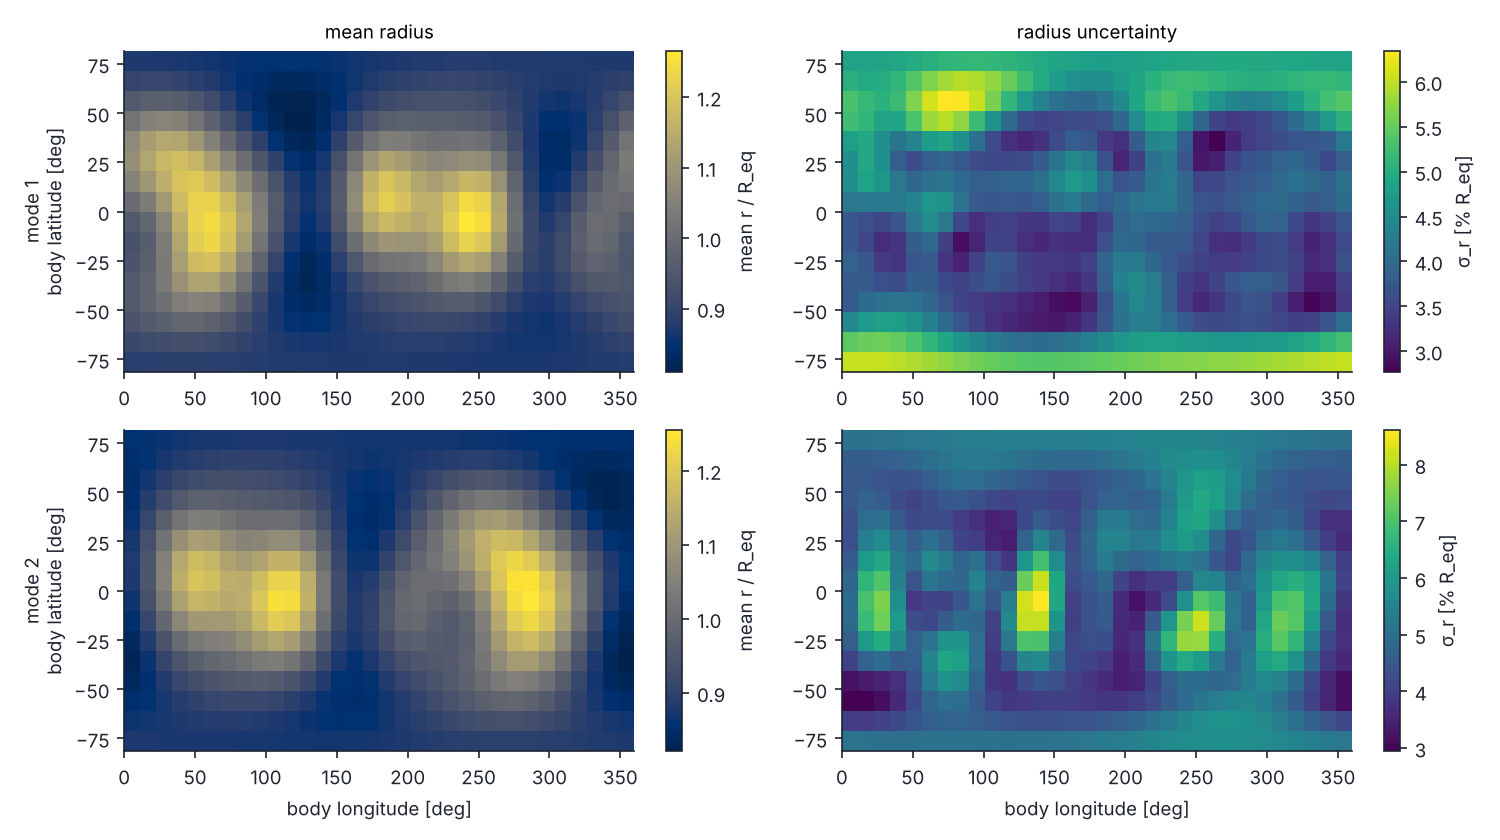
\includegraphics[width=\linewidth]{figures/fig_radius_maps.png}
  \caption{Mean radius (left) and radius standard deviation (right) in body coordinates, in units of the
  volume-equivalent radius, for mode~1 (top) and mode~2 (bottom).}
  \label{fig:rmaps}
\end{figure}

\subsection{Prior sensitivity}
\label{sec:app_sens}
Table~\ref{tab:sens} gives the MAP poles and Laplace mode weights under alternative priors. The
preference for the prograde mode persists in every setting ($w_2=0.83$--$0.99$). The prograde MAP pole
is stable at $(58^\circ,+67^\circ)$--$(58^\circ,+68^\circ)$. The retrograde MAP longitude jumps from
$247^\circ$ to $166^\circ$ under the tighter $\sigma_f$ prior, a direct expression of the near-gauge
behaviour of $\lambda$ close to the ecliptic pole. The MAP jitter is insensitive to the priors
(11.0--11.1\,mmag).

\begin{table}[t]
\centering
\caption{Prior sensitivity: MAP poles and Laplace-evidence weights.}
\label{tab:sens}
\small
\begin{tabular}{@{}lcccc@{}}
\toprule
Setting & Mode 1 MAP pole & $w_1$ & Mode 2 MAP pole & $w_2$\\
\midrule
Baseline ($\nu=2$, $\sigma_f$ median 0.15) & -- & 0.18 & -- & 0.82\\
$\nu=1.5$ (weaker damping) & $(247^\circ,-81^\circ)$ & 0.018 & $(58^\circ,+67^\circ)$ & 0.982\\
$\nu=3$ (stronger damping) & $(247^\circ,-81^\circ)$ & 0.168 & $(58^\circ,+68^\circ)$ & 0.832\\
$\sigma_f$ median 0.08 (tighter) & $(166^\circ,-77^\circ)$ & 0.010 & $(58^\circ,+67^\circ)$ & 0.990\\
\bottomrule
\end{tabular}
\end{table}

\subsection{Rerun with the quaternion body frame (adopted)}
\label{sec:app_quat}

\paragraph{Optimisation.} With the frame of Eq.~\eqref{eq:quatframe}, the multi-start MAP values agree
far better: within 3.2~nats in mode~1 and 0.3~nats in mode~2, against 17 and 11~nats with the Euler
frame. Most of the apparent orientation basins of the first run were therefore artefacts of the twist
coupling. Both maxima are fully converged (gradient norms $\approx10^{-10}$, positive-definite
Hessians).

At the MAP, the Laplace standard deviation of the pole along its weakest direction grows from
0.007--0.027\,rad (Euler) to 0.20--0.25\,rad (quaternion). The Euler frame had turned the posterior into
a thin curved ridge, of which both the Laplace approximation and the sampler saw only a narrow slice.

\paragraph{Sampling and convergence.} Table~\ref{tab:quat} compares the two runs. We assess convergence
also on the sampled chart coordinates $(d_1,d_2)$ and on the pole's unit-vector components, because the
longitude is a poor convergence metric near $|\beta|=90^\circ$: small pole moves change $\lambda$ by
large amounts there.
\begin{itemize}[nosep]
\item The quaternion run has no divergences (Euler: 1 and 6).
\item The mean trajectory length drops in both modes.
\item In the dominant mode, the longitude R-hat improves from 1.29 (ESS 12) to 1.04 (ESS 207).
\item The traces (Fig.~\ref{fig:traces_quat}) show the chains passing directly over the ecliptic pole,
  visible as jumps of $\lambda$ between $\approx70^\circ$ and $\approx300^\circ$, a move the Euler
  frame effectively forbade.
\end{itemize}
Convergence is improved but not complete: R-hat ranges from 1.04 to 1.15 on the chart coordinates, with
ESS of 20--100. This reflects a genuinely elongated posterior. Its spread along the chart's major axis
is $\approx27^\circ$ (mode~2) and $\approx38^\circ$ (mode~1), against $2^\circ$--$12^\circ$ in the
Euler run. Such a posterior needs longer and more numerous chains than the 2$\times$400 draws used here.

\begin{table}[t]
\centering
\caption{Euler versus quaternion body frame: identical data, priors and sampler settings (two chains,
400+400 iterations). Chart coordinates are the sampled gnomonic $(d_1,d_2)$; spreads are standard
deviations of $\arctan d$ along the chart axes.}
\label{tab:quat}
\small
\begin{tabular}{@{}>{\raggedright\arraybackslash}p{0.34\linewidth}cccc@{}}
\toprule
 & \multicolumn{2}{c}{Mode 1 (retrograde)} & \multicolumn{2}{c}{Mode 2 (prograde)}\\
 & Euler & Quaternion & Euler & Quaternion\\
\midrule
MAP start spread [nats] & 17.1 & 3.2 & 11.2 & 0.3\\
Divergences & 1 & 0 & 6 & 0\\
Mean leapfrog steps & 127 & 117 & 71 & 81\\
$\widehat R$ / ESS: $\lambda$ & 1.13 / 39 & 1.14 / 34 & 1.29 / 12 & 1.04 / 207\\
$\widehat R$ / ESS: $\beta$ & 1.19 / 77 & 1.05 / 49 & 1.07 / 22 & 1.09 / 69\\
$\widehat R$ / ESS: $d_1$, $d_2$ & 1.19, 1.17 & 1.09, 1.11 & 1.07, 1.07 & 1.07, 1.15\\
Pole spread along chart axes & $3.7^\circ$, $1.3^\circ$ & $38^\circ$, $7.7^\circ$ & $12^\circ$, $2.8^\circ$ & $27^\circ$, $4.0^\circ$\\
Pole radius 68\% / 95\% & $3.8^\circ$ / $7.5^\circ$ & $24^\circ$ / $57^\circ$ & $9.0^\circ$ / $22^\circ$ & $19^\circ$ / $43^\circ$\\
Mean pole & $(247^\circ,-80^\circ)$ & $(241^\circ,-66^\circ)$ & $(69^\circ,+57^\circ)$ & $(69^\circ,+59^\circ)$\\
Laplace $\ln Z$ & 768.55 & 768.90 & 770.09 & 773.20\\
Mode weight & 0.18 & 0.013 & 0.82 & 0.987\\
\bottomrule
\end{tabular}
\end{table}

\begin{figure}[t]
  \centering
  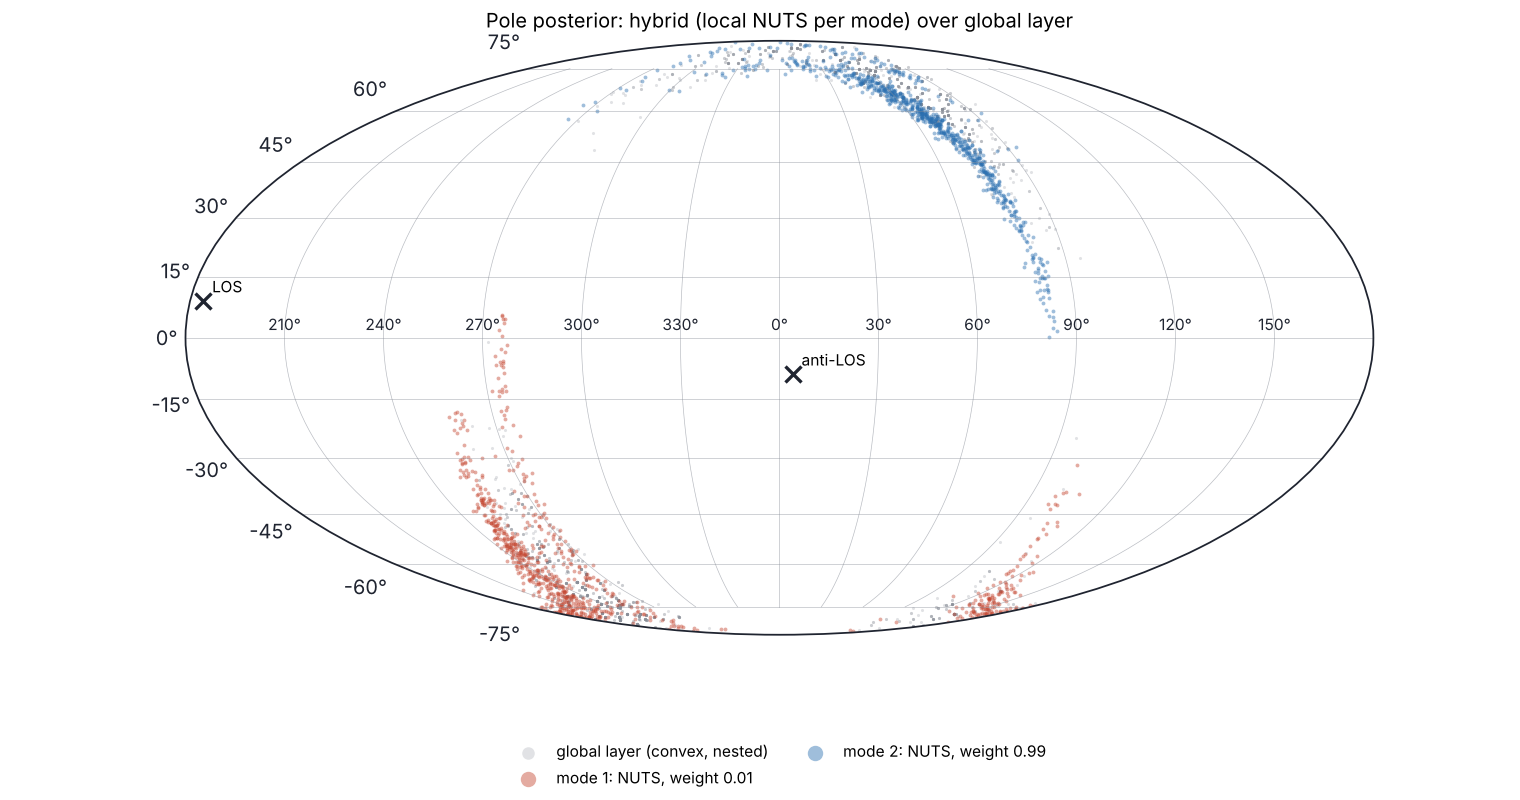
\includegraphics[width=\linewidth]{figures/fig_pole_hybrid_quat.png}
  \caption{Pole posterior with the quaternion body frame. Both modes extend along the great circle
  perpendicular to the line of sight, and the prograde mode carries 99\% of the evidence weight.}
  \label{fig:pole_quat}
\end{figure}

\begin{figure}[t]
  \centering
  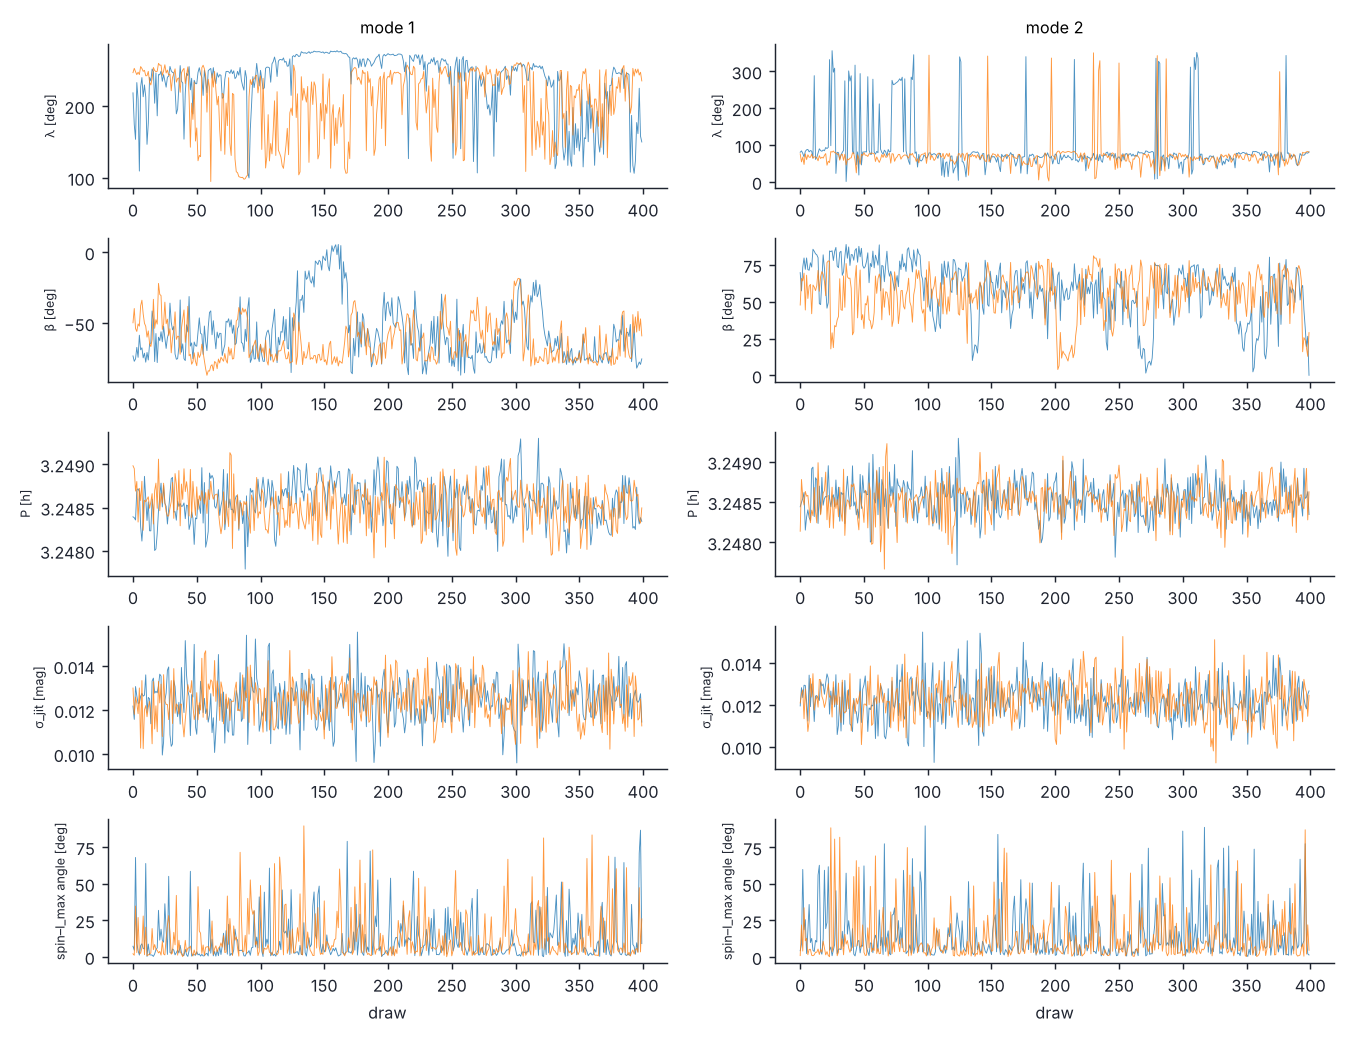
\includegraphics[width=0.75\linewidth]{figures/fig_traces_quat.png}
  \caption{NUTS traces with the quaternion frame. The jumps of $\lambda$ in mode~2 are passages over the
  ecliptic pole, which the Euler frame effectively forbade.}
  \label{fig:traces_quat}
\end{figure}

\paragraph{Posterior.} The adopted results (Fig.~\ref{fig:pole_quat}) are:
\begin{itemize}[nosep]
\item Both modes extend along the arc of the great circle perpendicular to the line of sight. This is
  the degeneracy expected when a single apparition constrains the pole mainly through the requirement
  of near equator-on viewing.
\item The prograde mode, centred at $(69^\circ,+59^\circ)$, carries Laplace weight 0.987. This exceeds
  the Euler run's 0.82 and the 0.83--0.99 range of the prior-sensitivity analysis. PSIS-LOO agrees in
  sign ($873.3\pm14.2$ against $871.2\pm14.1$), with all Pareto $\hat k<0.5$.
\item The sidereal period is $3.24853$ ($3.24830$--$3.24874$)\,h in mode~2
  and $3.24856$ ($3.24831$--$3.24878$)\,h in mode~1.
\item The jitter is $12.2$ ($11.2$--$13.2$)\,mmag.
\item The principal moments are $0.665:0.972:1$, with a median spin--maximum-inertia tilt of
  $7^\circ$ ($2^\circ$--$26^\circ$, moment gap 0.028).
\item The median radius uncertainty is $4.5\%\,\Req$.
\end{itemize}
The physical checks are similar to the first run. The shapes remain non-convex (median protrusion
$0.17$--$0.20\,\Req$), with ray-traced self-shadowing errors of $5.2$--$5.7$\,mmag rms and maxima of
17--21\,mmag.


%==========================================================================================
\section{Discussion}
\label{sec:discussion}

\paragraph{What the hybrid layer changes.} Compared with the convex analysis of the same data
\citep{lcinv_convex2026}, the radius-field model with an inertia prior produces shapes that rotate
about their axis of maximum inertia to within a few degrees. It fits the data better (jitter $12$
versus $17$\,mmag; the gain partly reflects the extra freedom of a non-convex surface). It also shifts
the mirror-mode weights from about even to strongly favour the prograde solution: $0.82$ with the Euler
frame and $0.987$ with the quaternion frame. The preference is robust to the shape-prior settings and
consistent in sign with PSIS-LOO. That the mode
weights depend on the shape model at all is itself an important result. For a single apparition the
mirror ambiguity is broken only by small departures from coplanar geometry, so its resolution is
model-dependent and should not be over-interpreted.

\paragraph{Pole mixing: an approximate gauge near the ecliptic pole, and its resolution.} The poor
mixing of the first run had a geometric cause, not a statistical one. The Euler body frame twists about
the spin axis at a rate $\tan\beta$ per unit pole displacement (Proposition~\ref{prop:twist}). Because
the shape harmonics absorb any twist, the likelihood acquires a long, curved, nearly flat ridge between
pole and shape orientation, which makes HMC saturate its tree depth or diverge. The gnomonic chart
removes the coordinate singularity of the \emph{pole}, but not this coupling, which enters through the
construction of the \emph{body frame}.

The quaternion parallel-transport frame of Eq.~\eqref{eq:quatframe} bounds the twist rate by
$\tan(d/2)$ around the mode centre (Proposition~\ref{prop:qtwist}). In the rerun this removed all
divergences and collapsed the spurious MAP basins. It let the chains cross the ecliptic pole freely, and
it improved the longitude R-hat of the dominant mode from 1.29 to 1.04 (\S\ref{sec:app_quat}).

Its most important effect is to reveal how broad the pole posterior actually is. The Euler run's pole
intervals were too narrow by a factor of 2--10, because the chains were confined to a slice of the
ridge. That broad, elongated posterior now determines the remaining sampling cost. Reaching R-hat
$<1.01$ needs longer and more chains; on a GPU these can be vectorised cheaply. Alternatively, the chart
axes can be aligned with the great circle perpendicular to the line of sight, which would make the
posterior nearly axis-aligned for the dense mass matrix.

\paragraph{Non-convexity and the scattering sum.} The posterior shapes are far from convex in the
facet-plane sense. Their self-shadowing errors ($\approx6$\,mmag rms, up to 30\,mmag) are comparable to
half the jitter, so part of the fitted jitter may be model error from Eq.~\eqref{eq:brightness}. The
local-dent penalty is too weak to prevent this, because it acts on a coarse vertex stencil and with a
loose scale. Three remedies are possible:
\begin{itemize}[nosep]
\item a stronger, facet-plane convexity prior, tested against the ray-traced error;
\item a differentiable approximation of self-shadowing, e.g.\ horizon maps on the radius grid, in the
  forward model;
\item importance re-weighting of the NUTS draws with the ray-traced likelihood, which is exact but
  efficient only while the shadowing errors remain small.
\end{itemize}
Because non-convexity is only weakly constrained by photometry \citep{durech2003}, a convexity prior is
also a defensible default.

\paragraph{Other approximations.} The $16\times32$ mesh contributes $\approx2.4$\,mmag rms
discretisation error; a $24\times48$ mesh halves it at twice the cost. The mode weights rest on Laplace
evidences, which are adequate when each mode is close to Gaussian but untested here against
thermodynamic integration. The pointwise LOO terms are evaluated at the draw-wise profiled offsets.

\paragraph{Conclusions.} The two-layer design does what it was built for:
\begin{itemize}[nosep]
\item the global layer finds and pre-weights the mirror modes;
\item the local layer delivers physically admissible shapes with joint spin--shape uncertainties and an
  internally consistent model comparison;
\item the diagnostics expose the remaining weaknesses rather than hiding them, as the frame-twist
  coupling showed.
\end{itemize}
For 2003~QN$_{21}$ the robust conclusions are the period $P=3.2485\pm0.0002$\,h, the near equator-on
viewing, an elongated shape with moments $\approx0.66:0.97:1$, and a model-dependent preference ($w\approx0.99$) for a prograde pole. That pole lies on an arc around
$(69^\circ,+59^\circ)$ with a 68\% radius of $\approx19^\circ$, extending along the great circle
perpendicular to the line of sight. A definitive pole requires longer chains, a convexity-consistent
forward model, and, most importantly, photometry from additional apparitions, which would cut the arc
down to a point.


\section*{Software}
The implementation (\texttt{lcinv.hybrid}) uses JAX \citep{jax2018}, Optax \citep{optax2020}, NumPyro
\citep{phan2019}, ArviZ \citep{kumar2019}, \texttt{dynesty} \citep{speagle2020}, Astropy
\citep{astropy2022} and \texttt{astroquery} \citep{ginsburg2019}.

\bibliographystyle{plainnat}
\bibliography{references}

\appendix
\section{Settings}
\label{app:settings}
\small
\begin{tabular}{@{}>{\raggedright\arraybackslash}p{0.40\linewidth}>{\raggedright\arraybackslash}p{0.56\linewidth}@{}}
\toprule
Item & Default\\
\midrule
Harmonic degrees $l_{\min}$--$l_{\max}$; coefficients $k$ & 2--5; 32\\
Grid $N_\vartheta\times N_\varphi$; vertices; triangles & $16\times32$; 514; 1024\\
Spectrum exponent $\nu$; hyperpriors & 2; $\ln\sigma_f\sim\mathcal N(\ln0.15,0.5^2)$, $\ln\ell\sim\mathcal N(\ln3,0.5^2)$\\
Scattering & Lommel--Seeliger $+\,0.1$ Lambert; softplus $T=0.005$\\
Inertia prior $s_{\mathrm{off}}$, $s_{\mathrm{ord}}$; convexity $s_{\mathrm{cvx}}$ & 0.005, 0.005; 0.02\\
Jitter prior & $\ln\sigma_{\mathrm{jit}}\sim\mathcal N(\ln0.015,1)$\\
Period prior & $P_0+\sigma_Pz_P$, $z_P\sim\mathcal N(0,1)$\\
MAP & L-BFGS, 4 starts, 2000 iterations\\
NUTS & 2 chains, 400 warm-up + 400 draws, target acceptance 0.9, max tree depth 7, dense mass\\
\bottomrule
\end{tabular}

\section{Algorithm}
\begin{enumerate}[leftmargin=*]
\item Run the global layer \citep{lcinv_convex2026} and obtain equal-weight pole samples, $P_0$ and $\sigma_P$.
\item Identify modes by density clustering on $\Sph$ (\S\ref{sec:modes}).
\item For each mode $k$:
  \begin{enumerate}[nosep]
  \item build the local model with the gnomonic chart centred on $\uv p_k$;
  \item find the multi-start MAP and verify $\lVert\nabla\rVert\approx0$ and $\mathsf H\succ0$;
  \item compute $\ln Z_k$ and $\mathsf H_k^{-1}$ (Eq.~\ref{eq:laplaceZ});
  \item run NUTS initialised from the Laplace approximation;
  \item compute derived quantities (pole, period, jitter, hyperparameters, inertia tilt and moments,
    radii normalised by $\Req$, pointwise log-likelihood);
  \item compute $\widehat R$, ESS, divergences, LOO, convexity and ray-traced shadowing errors.
  \end{enumerate}
\item Set $w_k\propto Z_k$, form the mixture (Eq.~\ref{eq:mixture}) and run the prior-sensitivity
  analysis.
\end{enumerate}

\end{document}
